\chapter{Introduction}
\label{c:intro}

RuleWorks is a rules-based programming language that represents an
evolutionary step beyond OPS5. The major features of RuleWorks are
listed below:

\begin{itemize}
\item Improved data representation
\begin{itemize}
\item inheritance hierarchy
\item working memory can be partitioned
\end{itemize}
\item Improved program modularity
  \begin{itemize}
  \item programs can be divided into independent, or dependent,
    modular subsystems
  \item rules-based modules can easily be called, and can return a
    value
  \end{itemize}
\item Portable implementation supporting numerous platforms
\end{itemize}

OPS5 is a rules-based programming language that was used most often to
develop knowledge-based and expert systems. It was created at Carnegie
Mellon University in the late 1970s and early 1980s by Charles Forgy,
John McDermott, the late Allen Newell, and Mike Rychener. Publication
of Forgy's OPS5 User's Manual in 1981 established a commonly used
standard for the language. OPS5 is characterized by:

\begin{itemize}
\item A global database, called working memory.
\item Program statements called condition-action rules that match
  patterns in working memory and then perform actions that change
  working memory.
\item Execution order that is not procedural, but is driven by the
  data in working memory. The order in which rules are executed is
  controlled by the recognize-act cycle.
\item Computation with symbolic expressions and numbers.
\end{itemize}

\section{Sample Program}

Most of the examples in this guide are based on a sample program
called \tt{KIWI}, which solves the system configuration problems of a
hypothetical manufacturer, the Kiwi Computer Company. Kiwi Computer
Co. makes the computer parts shown in Table \ref{t:kiwi}. A customer
can order a Kiwi computer as a package or as separate parts. The
purpose of the \tt{KIWI} program is to help the Kiwi sales force
verify that the parts a customer has ordered can be assembled into a
working computer.

\begin{table}[h]
  \begin{tabularx}{\columnwidth}{lXr}
    \toprule
    Part Number &  Name &  Price (\$) \\
    \midrule
    KI-9200   & Kiwi-9200 CPU Base Unit & 999.95 \\
    MS-9200   & Kiwi-9200 Memory Card   & 129.95 \\
    FD-35     & 3.5-inch Floppy Disk Drive &  99.95 \\
    FD-525    & 5.25-inch Floppy Disk Drive & 109.95 \\
    HD-30     & 30-Megabyte Hard Disk Drive & 299.95 \\
    HD-200    & 200-Megabyte Hard Disk Drive & 599.95 \\
    TA-9200   & High-Performance Cartridge Tape & 399.95 \\
    KB-9200   & 108-Key Keyboard with Mouse Port &  99.95 \\
    MOUSE-1   & 100 pulses per inch Graphic Mouse & 59.95 \\
    VM-9200   & 19-inch B/W Alphanumeric Monitor &  99.95 \\
    CM-9200   & 21-inch Color Graphic Display System & 199.95 \\
    NI-9200   & Kiwi-9200 Network Interface &  39.95 \\
    S-OS-9200 & KIWOS Operating System & 9.95 \\
    S-WI-9200 & KiWindows Windows Software &  59.95 \\
    S-CA-9200 & KiwiCalc Spreadsheet Software  &  29.95 \\
    S-NE-9200 & KiwiTalk Network Software &  89.95 \\
    \bottomrule
  \end{tabularx}
  \caption{Parts Manufactured by Kiwi Computer Company}
  \label{t:kiwi}
\end{table}

\section{Working Memory}

\emph{Working memory} is a global, dynamic user workspace that
contains information about a problem and the current state of its
solution. Information is stored in \emph{working memory objects} that
are organized by \emph{class}.  Each working memory object (WMO,
pronounced ``wim-oh'') has a class name and a list of associated
\emph{attributes} and their values. The class name classifies the
object according to the type of information it contains. The
attributes and their values describe the object's characteristics. (In
database terms, object classes are like tables and attributes are like
fields).

The information in Table~\ref{t:kiwi} could be represented in working
memory by objects that are all instances of a single class, named
\tt{PART}. A better representation would use several classes to
capture more information about the differences between types of
parts. For example, most of the Kiwi parts are optional (a customer
can buy either a floppy disk drive or a hard disk drive) but one is
required (the base unit that contains the CPU). This distinction can
be represented by class \tt{OPTION} for the optional components and
class \tt{BOX} for the required CPU box.

RuleWorks allows object classes to be organized into an inheritance
hierarchy in which \emph{subclasses} inherit from a \emph{parent
  class}. In this example, \tt{OPTION} and \tt{BOX} are subclasses (or
\emph{descendants}) of the parent class \tt{PART} (see Figure~\ref{f:1-1}).

All parts made by Kiwi Computer Company have the following three
characteristics: a part number, a name, and a price. These
characteristics are represented by attributes whose names are
\tt{PART-NUMBER}, \tt{NAME}, and \tt{PRICE}. These attributes are
declared in object class \tt{PART} and are inherited by its
descendants.

\begin{figure}
  \centering
  \input f1-1.tex
  \caption{Class Hierarchy of Parts}
  \label{f:1-1}
\end{figure}

(Figure~\ref{f:1-1} shows only part of the class hierarchy used in the
sample program. For a complete illustration, see Figure 2-1)

Some of the optional parts are hardware; some are software. Hardware
and software have different characteristics and are therefore
separated into different classes with different attributes. For
example, a hardware component can take up a slot in the CPU box while
a software component does not.  Conversely, software is available on
different media (two sizes of floppy disk, or tape) while hardware is
not.

The software options can be further divided between applications and
the operating system. Kiwi Computer currently sells three
applications, so there are three subclasses of \tt{APPLICATION}. There
is currently only one subclass of \tt{OPERATING-SYSTEM}, but there may
be other supported operating systems in the future.

A sample object of class \tt{BOX} is shown below.  The first three
attributes are inherited from class \tt{PART} and have values from
Table~\ref{t:kiwi}. The last two attributes belong to class \tt{BOX}
only, because the box is the only part that has slots:

\begin{quote}
\begin{verbatim}
(box ^part-number ki-9200 ^name |Kiwi-9200 CPU Base Unit| 
     ^price 999.95 ^card-in-slot ^card-in-slot-obj-id)
\end{verbatim}
\end{quote}

The attribute names are preceded by a caret (\ct) to show that they
are references into the object.

\section{Rules}

Program statements in RuleWorks are condition-action (or ``if
\ldots{}then'') rules that operate on working memory. A \emph{rule}
has a name and consists of a condition part (called the
\emph{left-hand side} or LHS) and an action part (called the
\emph{right-hand side} or RHS). The LHS is separated from the RHS by
an arrow, created by typing two minus signs and a greater-than
sign. Figure~\ref{f:1-2} shows the format of a rule.

Rules express the requirements of the problem to be solved. For
example, one requirement of the Kiwi program is that a customer who
buys application software must also buy the \tt{KIWOS} operating
system. The rule shown in Example~\ref{e:samprule} enforces this
requirement. The left-hand side of the rule matches when the contents
of working memory do not meet the \tt{KIWOS} requirement; the
right-hand side of the rule takes corrective actions.

\begin{figure}[h]
  \centering
  \input f1-2.tex
  \caption{Format of a Rule}
  \label{f:1-2}
\end{figure}

\begin{exampl}
\begin{verbatim}
(rule
    verify-configuration:application-needs-kiwos
    (active-context ^name verify-configuration)
    (kiwos-application ^$instance-of <applic>)
    -(kiwos)
  -->
    (write
        (crlf) |Caution: to run an application| <applic>
        (crlf) |you need to have KIWOS, but you don't have KIWOS.|
        (crlf) | Fixup: adding KIWOS to your order.|
        (crlf))
    (make error ^severity warning ^message |No operating system|)
    (make kiwos))
\end{verbatim}
\label{e:samprule}
\end{exampl}

\subsection{The Left-Hand Side}

The LHS is a series of patterns called \emph{condition elements} (CEs)
that are compared to objects during program execution.  RuleWorks
implicitly performs a logical AND operation on all the CEs on the
LHS. (In database terms, each CE is like a query against a table, and
the LHS is a like a join across the results of those queries.)

The LHS of the sample rule in Example~\ref{e:samprule} consists of
three CEs. The first CE is used to control the flow of execution of
the program. It states that the program must be in the "verify
configuration" phase of execution before this rule can \emph{fire} (be
executed).

The second CE states that an object of class \tt{KIWOS-APPLICATION} or
any of its subclasses exists in working memory. The customer order
could include any application: \tt{KiWindows}, \tt{KiwiCalc}, or
\tt{KiwiTalk}. Because subclasses inherit \emph{membership} in their
parent classes, objects of classes \tt{KIWINDOWS}, \tt{KIWICALC}, or
\tt{KIWITALK} match the class name \tt{KIWOS-APPLICATION} (see
Figure~\ref{f:1-1}). The second CE also binds (assigns a value to) the
variable \tt{<APPLIC>}.

The third CE is negated. It states that no object of class \tt{KIWOS}
exists.

\subsection{The Right-Hand Side}

The RHS is a series of actions that are taken when the rule is
executed. Actions are taken in the order you write them. An action
consists of an action name and its arguments; it usually manipulates
the contents of working memory.

The RHS of the sample rule in Example~\ref{e:samprule} contains three
actions. The \tt{WRITE} action displays a message to the user that the
order is being changed. The variable \tt{<APPLIC>} that was bound on
the LHS is used here on the RHS. The two \tt{MAKE} actions create new
objects of the classes \tt{ERROR} and \tt{KIWOS}, respectively. The
creation of the \tt{KIWOS} object changes the contents of working
memory such that the operating system requirement is met. Thus, this
rule will fire only once even if the customer orders all three
applications.

\section{Recognize-Act Cycle}

The recognize-act cycle is the pattern-matching procedure that takes
place repeatedly as a RuleWorks program executes (see
Figure~\ref{f:1-3}). The cycle consists of the following steps:

\begin{center}
  \begin{tabularx}{\columnwidth}{cX}
    \textbf{Match}  & Search working memory to find
                      all combinations of objects
                      that satisfy the condition  
                      elements in the left-hand sides 
                      of the program's rules. A rule 
                      name plus a combination of     
                      objects that satisfy that     
                      rule's condition elements is    
                      called an \emph{instantiation}. Place 
                      all instantiations in a list   
                      called the \emph{conflict set}. [In   
                      database terms, the conflict    
                      set is like a collection of the 
                      results of all the joins        
                      (left-hand sides) in the
                      program.] \\\addlinespace
    \textbf{Select} & Using an ordered sequence of  
                      criteria, take the             
                      instantiation with the highest 
                      priority out of the conflict    
                      set. If the conflict set is     
                      empty (because no left-hand     
                      side has been satisfied), the   
                      cycle stops. \\\addlinespace
    \textbf{Act}    & Execute the actions on the      
                      right-hand side of the rule in  
                      the selected instantiation,     
                      operating on the objects       
                      matched by its left-hand side. 
  \end{tabularx}
\end{center}

You can think of the match and select steps together as recognizing
which is the best rule to fire, thus the term recognize-act cycle.

\begin{figure}[h]
  \centering
  \input f1-3.tex
  \caption{Recognize-Act Cycle}
  \label{f:1-3}
\end{figure}

The cycle can stop after the select step, if the conflict set is
empty. It stops during the act step if a \tt{RETURN} or \tt{QUIT}
action is executed.

\section{Conflict Resolution}

The process by which the run-time system selects one instantiation
from the conflict set is called \emph{conflict resolution}. During
conflict resolution, the run-time system uses one of two possible
strategies to select the best instantiation, based on five different
criteria (see Table~\ref{t:crc}).

\begin{table*}[h]
  \def\arraystretch{1.2}
  \begin{tabularx}{\columnwidth}{lX}
    \toprule
    \textbf{Refraction}   & Select an instantiation 
                            only once.               
                            Refraction prevents       
                            programs from looping    
                            infinitely on the same   
                            data by removing         
                            instantiations from the 
                            conflict set after they 
                            have been selected.  \\
    \textbf{Recency}      & Select the instantiation 
                            that refers to the most  
                            recent information.      
                            Objects that have the    
                            highest time-tags contain
                            the most recent data.    
                            Therefore, the system    
                            selects the instantiation 
                            that contains the highest
                            time-tags.              \\
    \textbf{Class Specificity} & Select the instantiation 
                                 whose rule refers to the 
                                 most specific class      
                                 names.                   
                                 Class specificity is     
                                 determined by the        
                                 position of object       
                                 classes in the           
                                 inheritance hierarchy.  
                                 Top-level classes are    
                                 less specific than       
                                 low-level classes. For   
                                 example, a \tt{PART} object is 
                                 least specific; a        
                                 \tt{KIWINDOWS} object is most 
                                 specific. \\
    \textbf{Test Specificity} &  Select an instantiation 
                                of the rule whose        
                                left-hand side is the    
                                most specific.          
                                Test specificity is     
                                determined by the number 
                                of attribute-value tests 
                                in the rule's left-hand  
                                side. The rule whose     
                                left-hand side contains 
                                the most tests is the    
                                most specific. \\
    \textbf{Arbitrary choice} &  After all other criteria 
                                have been applied and   
                                more than one            
                                instantination remains,  
                                select one at random. \\
    \bottomrule
  \end{tabularx}
  \caption{Conflict Resolution Criteria}
  \label{t:crc}
\end{table*}

The RuleWorks run-time system supports two conflict-resolution
strategies: the lexicographic-sort (\tt{LEX}) strategy and the
means-ends-analysis (\tt{MEA}) strategy. The \tt{LEX} strategy applies
each selection criterion once, in the order shown in
Table~\ref{t:crc}. The \tt{MEA} strategy follows the same order, but
it applies recency in two steps. First it selects the instantiation(s)
whose first time-tag is most recent. It then selects from the
remaining instantiation(s) the one(s) whose combined time-tags are
most recent.

The sample program, \tt{KIWI}, uses the \tt{MEA} strategy to create a
control structure. The program divides the problem into tasks, creates
an object for each task, and places the condition element that matches
the control object first on each left-hand side (see Example 1-1). The
extra step of the \tt{MEA} strategy ensures that only instantiations
that match the most recent control object can fire.

The default strategy for RuleWorks is \tt{MEA}, and DIGITAL recommends
using this strategy for almost all applications. You can change the
strategy to \tt{LEX} with the \tt{STRATEGY} clause of the
\tt{ENTRY-BLOCK} declaration.

\section{Other Program Components}

In addition to rules, RuleWorks programs consist of block constructs,
declarations, optional \tt{ON-} statements, optional catchers, and
optional comments. Each program must have at least one entry block;
declaration blocks and rule blocks are optional. Inside an entry
block, program statements must be ordered as shown in
Figure~\ref{f:1-4}: declarations first, then \tt{ON-} statements (if
any), last rules and catchers.

\begin{figure}[h]
  \centering
  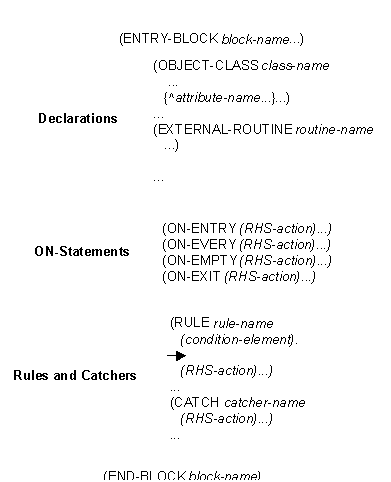
\includegraphics[scale=0.7]{f1-4}
  \caption{Format of a RuleWorks Program}
  \label{f:1-4}
\end{figure}

\subsection{Block Constructs}

RuleWorks provides block constructs for program and data
modularity. In OPS5, all rules were active and all of working memory
could be matched by any rule. In RuleWorks, the rules and WMOs of one
block can be isolated from those of every other block.

RuleWorks provides three block constructs:

\begin{tabularx}{\columnwidth}{lX}
    \toprule
    Name & Purpose \\
    \midrule
    \tt{ENTRY-BLOCK} & Makes an entry point
                       for your RuleWorks   
                       code so that it can  
                       be called from       
                       RuleWorks or other   
                       languages, accepting 
                       arguments and        
                       optionally returning 
                       a value. Objects     
                       whose class is       
                       declared inside an   
                       entry block can be   
                       matched by rules in  
                       that entry block     
                       only. \\\addlinespace
    \tt{DECLARATION-BLOCK} & Creates a collection
                             of object class and  
                             external routine     
                             declarations that    
                             can be shared among  
                             entry blocks.        
                             Objects whose class  
                             is declared inside a 
                             declaration block    
                             can be matched by    
                             rules in any entry   
                             or rule block that   
                             uses that            
                             declaration block. \\\addlinespace
    \tt{RULE-BLOCK} & Creates a collection
                      of rules that can be 
                      shared among entry   
                      blocks. Objects      
                      whose class is       
                      declared inside a    
                      rule block can be    
                      matched by rules in  
                      that rule block      
                      only. \\\addlinespace
    \bottomrule
  \end{tabularx}


Each block must end with an \tt{END-BLOCK} statement. See
Chapter~\ref{c:program} for more information on block constructs.

\subsection{Declarations}

Declarations are units of code that define the object classes and
external routines used in a program. Object class and external routine
declarations must precede any executable statement.

\subsection{\tt{ON-} Statements}

\tt{ON-} statements contain actions that are executed at particular
steps in the recognize-act cycle, without matching objects in working
memory. RuleWorks provides four \tt{ON-} statements:

\begin{center}
\begin{tabular}{ll}
    \toprule
    Name     & Time Executed               \\
    \midrule
    \tt{ON-ENTRY} & Before match step of first recognize-act cycle. \\
    \tt{ON-EVERY} & After act step of every cycle except the last one. \\
    \tt{ON-EMPTY} & After select step when the conflict set is empty. \\
    \tt{ON-EXIT}  & After act step of the last cycle.  \\
  \bottomrule
\end{tabular}
\end{center}

Like rules, \tt{ON-} statements must be enclosed in parentheses. They
must appear after declarations (if any) and before other executable
statements (that is, rules and catchers). For more information see
Chapter~\ref{c:program}.

\subsection{Catchers}

Catchers contain actions that are executed after a certain number of
recognize-act cycles have fired, without matching objects in working
memory. You specify the number of cycles in an \tt{AFTER} action. For
more information see Chapter~\ref{c:program}.

\subsection{Comments}

To improve the readability of your program, you can format units of
code by using white space (spaces, tabs, and new-line characters) and
comments. A comment starts with a semicolon and finishes at the end of
the same line. For example:

\begin{quote}
\begin{verbatim}
;This is a comment.
\end{verbatim}
\end{quote}

If you want more than one line of comment text, you must start each
line with a semicolon.

The compiler ignores the text of comments.  Therefore, comments can
contain any ASCII character and can start anywhere that a space
character is valid.

%%% Local Variables:
%%% mode: latex
%%% TeX-master: "rwug"
%%% End:
